\documentclass{article}
\usepackage{graphicx}

\title{Goldbach's Conjecture}
\author{Joyce Huang}

%% \blurb{Goldbach’s Conjecture is one of the most famous unsolved math problems in the world. It states that every even integer greater than two can be expressed as the sum of two primes.}

\begin{document}

\maketitle
\begin{center}
    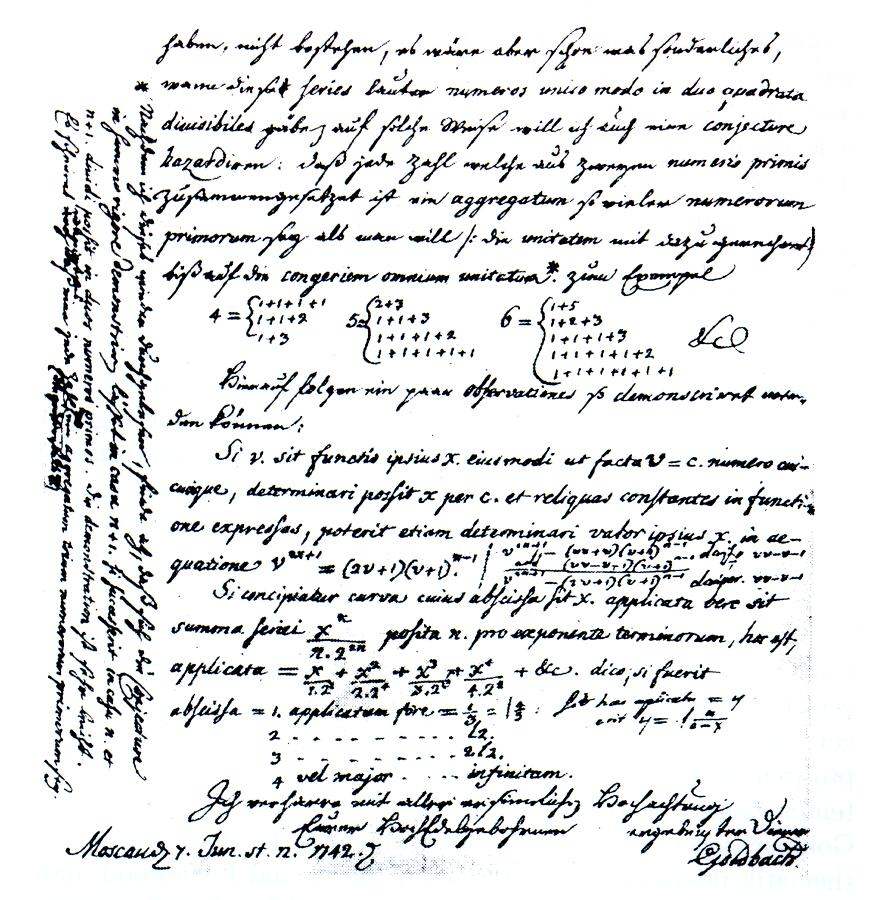
\includegraphics[width=4in,scale=0.18]{images/goldbach-conjecture.jpg}
\end{center}

Goldbach’s Conjecture is one of the most famous unsolved math problems in the world. It states that every even integer greater than two can be expressed as the sum of two primes. 

The conjecture is named after Christian Goldbach, a German mathematician who proposed it in 1742. On June 7th of that year, he wrote a letter to Leonhard Euler, another famous mathematician, that contained a conjecture he found: ``If an integer $n$ can be expressed as the sum of two primes, then it can also be expressed as the sum of $k$ primes, where $k$ is an integer from 2 to $n$.'' He also wrote a second conjecture in the margin of the letter: ``Every integer greater than 2 can be expressed as the sum of three primes.'' 

In Euler’s response letter, he recalled a previous conversation between the two, where Goldbach said that both of the above conjectures were results of another conjecture, ``Every even integer greater than 2 can be expressed as the sum of two primes,'' which is the final, strongest version of the conjecture.  

Even almost three hundred years after Goldbach first proposed his conjecture, it is still an open problem. Most mathematicians believe it to be true, and as of 2013, computers have confirmed it for numbers up to over $4\cdot10^{18}$ (4,000,000,000,000,000,000). 

One way some mathematicians have approached proving this conjecture is through the probabilistic method. The general idea is that as the even integer grows larger, there are more and more ways to express it as the sum of two integers, so the likelihood of there being at least one pair of two primes increases. While probability does not provide a rigorous proof, it has given strong evidence that large even numbers are the sum of not just one, but many pairs of primes.

In their exploration of this conjecture, mathematicians became interested in Goldbach’s function. Goldbach’s function outputs the number of ways to express an even integer as the sum of two primes. Its graph is pictured below:
\begin{center}
    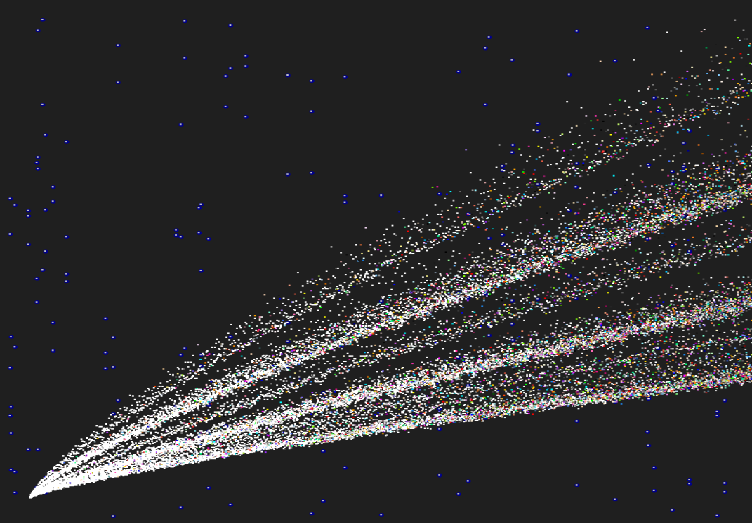
\includegraphics[scale=0.4]{images/goldbach-comet.png}
\end{center}
Mathematicians call the graph Goldbach’s Comet because the shape represents a comet and its tail. The streaks in the graph show that there are different groups of even integers whose number of ways to be expressed as the sum of two primes increase at different rates. The streaks are based off of the odd prime factors of the input. For example, the lowest streak consists of numbers who are either powers of 2 or can be expressed as $2p$, where $p$ is a prime number. Inputs of powers of 2 correspond to the lowest outputs because they are not divisible by any odd primes, which means if two odd numbers $a$, $b$ sum to the power of 2, they are never both divisible by any odd prime. Thus, the “ruling out” of pairs of odd numbers never overlaps, resulting in a smaller output. Furthermore, the groups appear to increase linearly.

Despite all the evidence suggesting that Goldbach’s conjecture is true, it is important to remember that it has not yet been proven, and we won’t know for sure until someone proves it. That someone could be anyone. It could even be you!
\begin{center}
    
\includegraphics[width=4in,scale=0.3]{images/stick_figure1.png}
\end{center}
\end{document}